% Typeset with XeTeX
% Allows use of system fonts rather than just LaTeX's ones
% NOTE - if you use TeXShop and Bibdesk (Mac), can complete citations
%  - open your .bib file, type~\citep{xx... and then F5 or Option-Escape
\documentclass[11pt]{article}
\usepackage[width=6.5in,height=10in]{geometry} % set page layout
\geometry{a4paper}  % or a4paper
\usepackage[xetex]{graphicx} % allows us to manipulate graphics.
% Replace option [] with pdftex if you don't use Xe(La)TeX
\usepackage{color}
\usepackage{indentfirst}
\usepackage{epstopdf} % automatic conversion of eps to pdf 
\usepackage{amsmath, amssymb} % Better maths support & more symbols
\usepackage{textcomp} % provide lots of new symbols - see textcomp.pdf
% line spacing: \doublespacing, \onehalfspacing, \singlespacing
\usepackage{setspace}
\singlespacing
\usepackage{pgfplotstable}
% allows text flowing around figs
% use \begin{wrapfigure}{x}{width} where x = r(ight) or l(eft)
\usepackage{wrapfig}
\usepackage[parfill]{parskip} % don't indent new paragraphs
\usepackage{flafter}  % Don't place figs & tables before their definition 
\usepackage{verbatim} % allows \begin and \end{comment} regions
\usepackage{booktabs} % makes tables look good
\usepackage{bm}  % Define \bm{} to use bold math fonts
% linenumbers in L margin, start & end with \linenumbers \nolinenumbers,
\usepackage{lineno} % use option [modulo] for steps of 5
\usepackage[auth-sc]{authblk} % authors & institutions - see authblk.pdf
\renewcommand\Authands{ and } % separates the last 2 authors in the list
% control how captions look; here, use small font and indent both margins by 20pt
\usepackage[small]{caption} 
\setlength{\captionmargin}{20pt}
%:FONT
% If you don't want to use system fonts, replace from here to 'Citation style' with \usepackage{Palatino} or similar
\usepackage[no-math]{fontspec} % 'no-math' = keep computer modern for math fonts unless you say differently below
\usepackage{xunicode} % needed by XeTeX for handling all the system fonts nicely
\usepackage[no-sscript]{xltxtra} 
\setmonofont[Scale=0.8]{PT Serif} % typeface for \tt commands
\setsansfont[BoldFont={PT Serif Bold}, ItalicFont={PT Serif Italic}]{PT Serif} %my choice of sans-serif font
\defaultfontfeatures{Mapping=tex-text} % convert LaTeX specials (``quotes'' --- dashes etc.) to unicode, to preserve them
% Main font: choose one of the following or build your own
% (most of these come with Mac OS X)
% Not all fonts come with a small-caps (\textsc) face so I use Palatino for small caps,
%  if necessary - this is a monstrous typographic hack
%
% Leave all the following lines commented to get the normal Latex Computer Modern font
%
%\setmainfont[BoldFont={Palatino Bold}, ItalicFont={Adobe Jenson Pro Italic}]{Adobe Garamond Pro}

\setmainfont{Adobe Garamond Pro}
%\setmainfont{Minion Pro}


%:CITATION STYLE
% natbib package: square,curly, angle(brackets)
% colon (default), comma (to separate multiple citations)
% authoryear (default),numbers (citations style)
% super (for superscripted numerical citations, as in Nature)
% sort (orders multiple cites into order of appearance in ref list, or year of pub if authoryear)
% sort&compress: as sort, + multiple citations compressed (as 3-6, 15)
\usepackage[numbers,comma,sort&compress]{natbib}

%:SHORTCUT COMMANDS
% Maths
\newcommand{\ddt}[1]{\ensuremath{\frac{{\rm d}#1}{{\rm d}t}}}  % d/dt
\newcommand{\dd}[2]{\ensuremath{\frac{{\rm d}#1}{{\rm d}#2}}} % dy by dx  - \dd{y}{x}
\newcommand{\ddsq}[2]{\ensuremath{\frac{{\rm d}^2#1}{{\rm d}#2^2}}} % second deriv
\newcommand{\pp}[2]{\ensuremath{\frac{\partial #1}{\partial #2}}} % partial \pp{y}{x}
\newcommand{\ppsq}[2]{\ensuremath{\frac{\partial^2 #1}{\partial {#2}^2}}}
\newcommand{\superscript}[1]{\ensuremath{^{\textrm{#1}}}} %normal (non-math) font for super/subscripts in text
\newcommand{\subscript}[1]{\ensuremath{_{\textrm{#1}}}}
\newcommand{\positive}{\ensuremath{^+}}
\newcommand{\negative}{\ensuremath{^-}}
% Editing
\newcommand{\red}[1]{{\color{red}{#1}}}
\newcommand{\redtext}[1]{{\color{red}{#1}}}
\newcommand{\blue}[1]{{\color{blue}{#1}}}
\newcommand{\bluetext}[1]{{\color{blue}{#1}}}
\newcommand{\scinot}[2]{\ensuremath{#1 \times 10^{#2}}}
% Standard stuff
\newcommand{\be}{\begin{equation}}
\newcommand{\ee}{\end{equation}}
\newcommand{\bea}{\begin{eqnarray}}
\newcommand{\eea}{\end{eqnarray}}

% \begin{graybox} text \end{graybox} for text with a background colour
\definecolor{MyGray}{rgb}{0.96,0.97,0.98}
\definecolor{MyGray}{rgb}{0.96,0.90,0.98}
\makeatletter\newenvironment{graybox}{%
	\begin{lrbox}
	{\@tempboxa}\begin{minipage}[r]{0.98\columnwidth}}{\end{minipage}\end{lrbox}%
	\colorbox{MyGray}{\usebox{\@tempboxa}}
}\makeatother


%%%%%%%%%%%%%%%%%%%%%%%

\title{B cell analysis}
\author{}

\date{}

\begin{document} 
\maketitle

\section*{Intrduction}
We are interested in studying the development and homeostatic maintenance of B cell subsets.
B cell development starts in the bone marrow and continues in periphery in spleen. In the spleen, immature B cells pass through 2 transitional stages T1 and T2 (identified based on AA44.1 expression) before maturing into functional B cell subsets.
Conventionally it is belived that T1 cells transition to T2 cells which then give rise to folicular mature (FM) and marginal zone (MZ) cells.
T2 cells and folicular mature cells circulate between spleen and lymph nodes while T1 and MZ cells are resticted to spleen only. Folicular mature cells participate in the germinal center reaction and give rise to germinal center GC cells.

\blue{Development and dynamics of GC B cells may be influenced by GC T cells and the kinetics of antigen decay. GC rection on an average lasts for $\sim$ 3 weeks.}


\textbf{Data:} \\
1. kinetics of Cell counts and donor fractions in Busulfan-chimeric mice. \\
Busulfan system allows us to track replacement of old host cells by new donor-derived B cells. Tracking chimerism dynamics in different B cell subsets helps us understand how B cells trickle down the developmental pathway itno diverse cell fates.\\

2. Ki67 expression within host and donor cells in busulfan chimeras.\\
Changes in the proportions of ki67 exressing cells helps us unravel life-death decisions between different cell subsets. 


\section*{Modelling Source influx} 
Rather than bulding a mechaistic model of influx of precursor cells, we used a spline that reasonably describes the shape of timecourse of the precursor population.
The rate of decline of source population over time $\rightarrow \nu$  is estimated by fitting the spline described in eq.~\ref{eq:source} to the cell counts of parent population.

\be
\phi(t) = \Phi \, e^{-\nu \, t}
\label{eq:source}
\ee


\paragraph*{Transitional 2 cells:} $\\$
Splenic T1 cells are considered as the only source for Transitional 2 cells.
Since, T2 cells circulate between spleen and LN, pooled counts of spleen + LN T2 cells were used for all fittings.
Donor chimerism in T1 cells stabilises by day 12 post BMT $\Rightarrow \, t_0$ for T2 anlysis using T1 as a source is day 12. 

\paragraph*{Folicular mature and Marginal zone cells:} $\\$
1. Pooled counts of (spleen + LN) T2 cells, \\
2. Splenic T1 cells \\
were used as precursors for the anlysis of pooled FM (spleen + LN) cells and splenic MZ cells.

Donor chimerism in T1 cells stabilises by day 12, however, in order to keep the number of observation identical, when comparing model fits from these 2 source populations, $t_0$ was adopted depending on the stabilisation of chimerism in T2 population, which is day 33.
 
\paragraph*{Germinal center cells:} $\\$
1. Pooled counts of (spleen + LN) FM cells, \\
2. Splenic MZ cells \\
were considered as precursors for the spleen GC cells. 

Only Pooled counts of (spleen + LN) FM cells were considered as precursors for LN GC cells. 

Donor chimerism in FM cells stabilises by day 67.


\begin{figure}[h!]
	\centerline{\includegraphics[scale = 1] {source.pdf}}
	\caption{Splines fitted Precursor population. Rate of change of source influx was estimated from the fitted spline for the respective source population. \label{fig:source}}
\end{figure}


\section*{Mathematical models describing B cell dynamics}

\paragraph*{Simple Homeogneous model:}
All cells behave identically at all times. \\
In this model we assume that cells follow random birth-death processes to form a kinetically homogeneous population that self renews through homeostatic division and decays either by death or maturation. 
Per capita net loss rate `$\lambda$' is given by loss - proliferation ($\delta - \rho$)  and is assumed to be constant over time. \\
Abbereviated as SHM

\be
\frac{dN}{dt} = \phi[t] \, - \lambda \, N(t)
\label{eq:SHM}
\ee

\paragraph*{Time-dependent model:} 
All cells behave identically at a given instant of time. \\
This is also a homogeneous model where all cells obey the same rules of turnover. We assume that the fitness of the whole population changes over time/host-age, due to host-intrisic factors. 
The net loss rate $\lambda$ varies with time. We explored different forms of lambda changing with time and the best-fit was obtained with the very general form representing slow exponential decline in $\lambda$ with host age, $\lambda(t) = \lambda_0 \, e^{-r\,t}$.
Abbereviated as TDM

\be
\frac{dN}{dt} = \phi[t] \, - \lambda(t) \, N(t)
\label{eq:TDM}
\ee


\paragraph*{Age-structured model:} 
This is a heterogeneous model where the ability of individual cells to die or divide varies with the time spent since the last developmental state. 
The net loss rate $\lambda$ is a function of cell's age in the current lineage. 
Changes in fitness of individual cells with age could possibly be a result of adaptive changes in cell-intrisic factors and/or conditioning that cells receive through micro-environmental inteactions (host intrisic factors).
Different forms of lambda were explored and the best-fit was obtained by, $\lambda(a) = \lambda_0 \, e^{-r \,a} $.
The PDE described in eq.~\ref{eq:ASM} tracks the population dynamics of $N(a,t)$ over time.
We also assume that the fitness of individual cells is inherited by their daughter cells.
Abbereviated as ASM

\be
\frac{\partial{N(a,t)}}{\partial{a}} + \frac{\partial{N(a,t)}}{\partial{t}} = - \lambda(a) N(a,t),
\label{eq:ASM}
\ee


\clearpage
\section*{Transitional 2 cells}

\paragraph{Summary}
\begin{itemize}
	\item Both homogeneous models, TDM and SHM, provide equally good visual descriptions of the data (Figure~\ref{fig:T2_T1}), but the \textbf{time-dependent model} was favoured statistically ($\Delta$AIC = 3.45, Table~\ref{tab:T2-AICs}).
	
	\item Age-strutured model fails to capture the kinetics of donor fractions (Figure~\ref{fig:T2_T1}), and therefore has significantly lower statistical support too ($\Delta$AIC = 13, Table~\ref{tab:T2-AICs}). This is expected, since we see complete replacement of host cells by that of donor derived cells, suggesting absence of heterogeneity.
	
	\item Estimates of net loss rate $\lambda(t)$ from the best-fit model i.e. TDM were plotted against host-age (Figure~\ref{fig:lambda}A). These estimates were used to derive the inter-division time and residence time of cells in T2 stage (Figure~\ref{fig:rates}A). These predictions suggest that T2 cells are very short lived and their rates of division and death do not change over time. Therfore, the kinetics of proportions of ki67Hi cells in T2 cells are purely driven by the changes in ki67 proportions in the source i.e. in T1 cells. 
	
\end{itemize}


%: Table T2
\begin{table}[h!]
	\begin{center}
		\renewcommand{\arraystretch}{1.25}
		\begin{tabular}{ l c c c } 
			\toprule 
			\multicolumn{1}{l}{\textbf{Pooled T2 cells using}} & \multicolumn{3}{c}{\textbf{Model and $\Delta$AIC}} \\
			\cline{2-4}
			\textbf{Source}  &  {\small Time-dependent}  &  {\small Age-structured} & {\small Simple-homogeneous} \\ 
			\toprule
			Splenic Transitional 1 cells      & 0      &  12.99 & 3.45  \\ 
			\hline
			\toprule 
		\end{tabular}
	\end{center}
	\caption{\small Comparison of AIC values for different models fitted to cell counts and donor fractions$^{\dagger}$ in Transitional 2 B cells (Spleen + LN).}
	$^{\dagger}$ \footnotesize{Donor fractions in T2 pool were normlised to the donor fractions in Splenic T1 population. }
	\label{tab:T2-AICs}
\end{table} 

\footnotesize{For model comparison only differences in AIC, not absolute values, are meaningful -- these differences are shown relative to the best-fitting model. A measure of the relative support for two models is exp$(- \Delta\text{AIC}/2)$.}

\begin{figure}[h!]
	\centerline{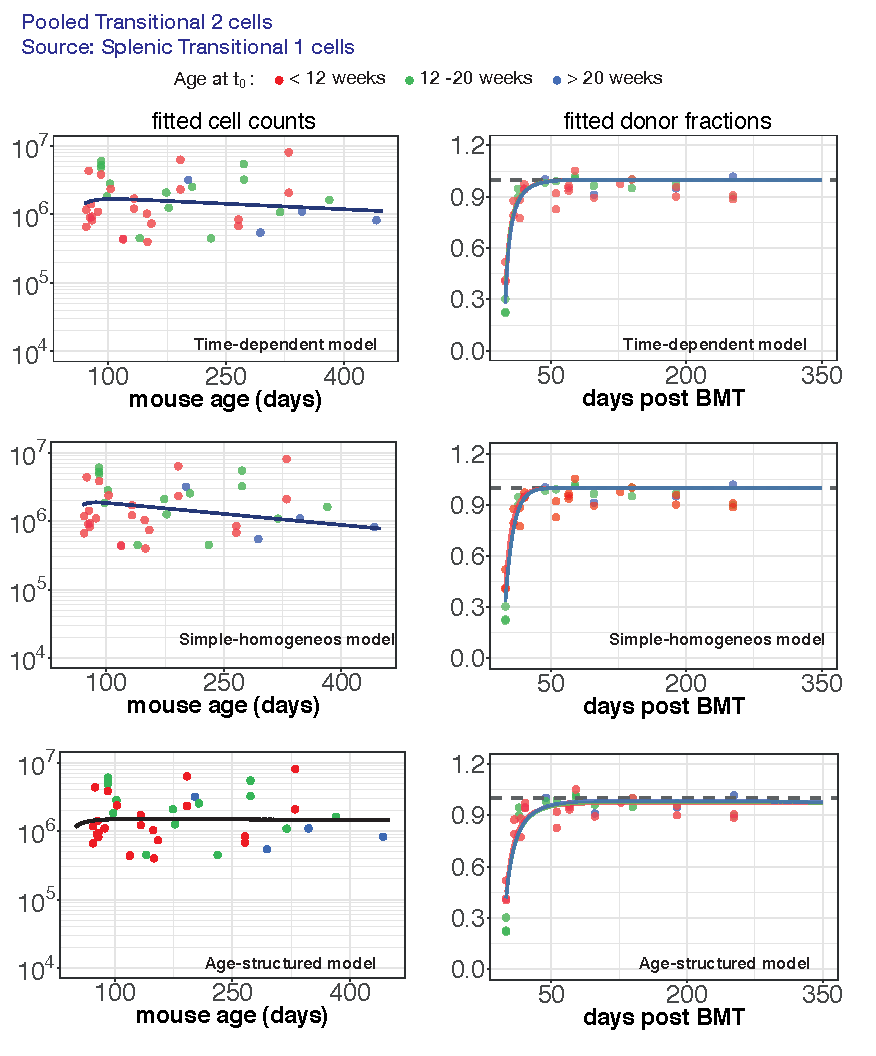
\includegraphics[scale = 1.1] {T2_T1.pdf}}
	\caption{\small \textbf{Comparison of models  explaining dynamics of T2 B cells considering splenic T1 cells as precursors, in busulfan chimeras.} The time-dependent, simple-homogeneous and age-structured$^{\dagger}$ models fitted simultaneously to T2 cell counts and the normalised chimerism from busulfan chimeras made in recipients of different ages. Colours indicate different age-groups of recipient mice. The predictions shown were generated using the  mode of the age within each group.}
	\label{fig:T2_T1}
\end{figure}


\clearpage


\section*{Folicular mature cells}


\paragraph{Summary}
\begin{itemize}
	\item We find that \textbf{time-dependent model} using \textbf{splenic Transitional1} cells as the source provides best descriptions of the cell counts and normalised donor fractions of the Pooled (spleen + LN) Folicular Mature cells (Figure~\ref{fig:FM_T1}), and was most favoured statistically (Table~\ref{tab:FM-AICs}).
	
	\item Again, the normalised donor fractions saturate to 1, suggesting homogeneity within FM population. Therefore, the age-strutured model that assumes heterogeneity fails to explain the data (Figure~\ref{fig:FM_T1}), and has lower statistical support. (Table~\ref{tab:FM-AICs}). 
	
	\item Interestingly, the simple-homogeneous model also has substantially inferior statistical support with respect to TDM. Probably, because of the poor descriptions of trends in cell counts with host age. 
	
	\item Host-intrisic factors control the population dynamics of FM cells.
	
	\item Changes in $\lambda(t)$ from the best-fit model i.e. TDM were plotted against host-age (Figure~\ref{fig:lambda}B). The inter-division and residence times of FM cells were inferred from the estimates of $\lambda(t)$ (Figure~\ref{fig:rates}B). We find that the FM cells are relatively long-lived (compared to MZ and T2).
	The rates of division and death of FM cells change gradually with time with a marked increase in old ages.
	
	\item The changes in the proportions of ki67Hi cells in the FM compartment can be attributed to, \\
	(i) the changes in ki67 proportions in the source i.e. in T1 cells and \\
	(ii)by the time-dependent changes in their division and death rates.
	
	
\end{itemize}

%: Table FM
\begin{table}[h!]
	\begin{center}
		\renewcommand{\arraystretch}{1.25}
		\begin{tabular}{ l c c c } 
			\toprule 
			\multicolumn{1}{l}{\textbf{FM cells using}} & \multicolumn{3}{c}{\textbf{Model and $\Delta$AIC}} \\
			\cline{2-4}
			\textbf{Source}  &  {\small Time-dependent}  &  {\small Age-structured} & {\small Simple-homogeneous} \\ 
			\toprule
			Splenic Transitional 1 cells      & 0      &  30.22  & 22.68  \\ 
			Pooled Transitional 2 cells       & 27.28  &  29.76  & 30.75  \\
			\hline
			\toprule 
		\end{tabular}
	\end{center}
	\caption{\small Comparison of AIC values for different models fitted to cell counts and donor fractions$^{\dagger}$ in Folicular Mature B cells, considering different precursor populations.}
	$^{\dagger}$ \footnotesize{Donor fractions in FM pool were normlised to the donor fractions in the respective source population. }
	\label{tab:FM-AICs}
\end{table} 




\begin{figure}[h!]
	\centerline{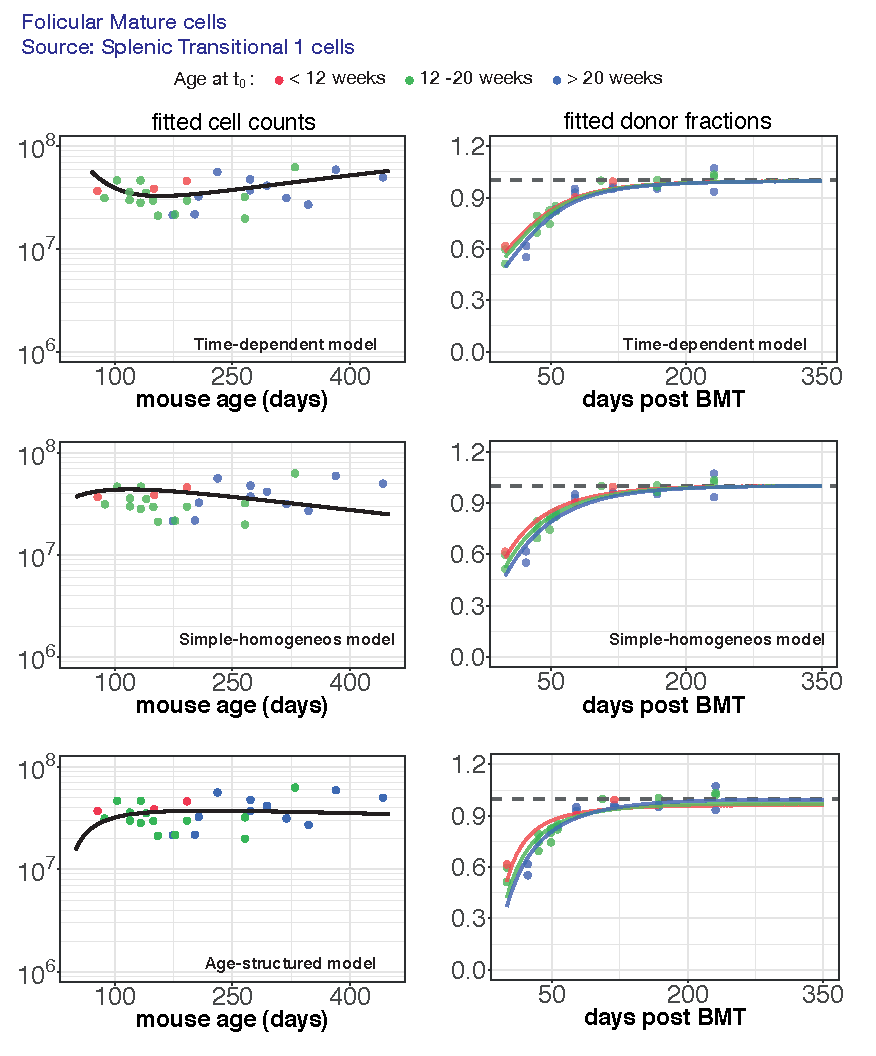
\includegraphics[scale = 1.1] {FM_T1.pdf}}
	\caption{\small \textbf{Comparison of models  explaining dynamics of FM B cells considering splenic T1 cells as precursors, in busulfan chimeras.} The time-dependent, simple-homogeneous and age-structured$^{\dagger}$ models fitted simultaneously to FM cell counts and the normalised chimerism from busulfan chimeras made in recipients of different ages. Colours indicate different age-groups of recipient mice. The predictions shown were generated using the  mode of the age within each group.}
	\label{fig:FM_T1}
\end{figure}

\begin{figure}[h!]
	\centerline{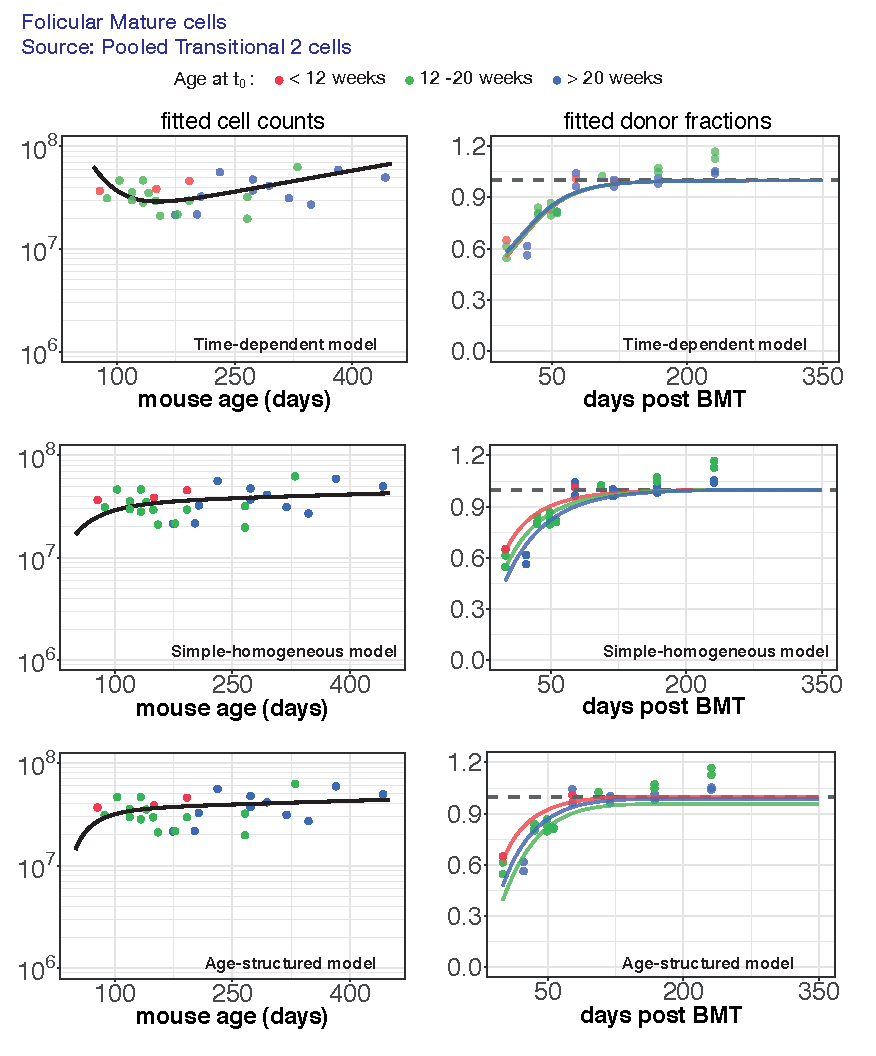
\includegraphics[scale = 1.1] {FM_T2.pdf}}
	\caption{\small \textbf{Comparison of models  explaining dynamics of FM B cells considering Pooled (spleen + LN) T2 cells as precursors, in busulfan chimeras.} The time-dependent, simple-homogeneous and age-structured$^{\dagger}$ models fitted simultaneously to FM cell counts and the normalised chimerism from busulfan chimeras made in recipients of different ages. Colours indicate different age-groups of recipient mice. The predictions shown were generated using the  mode of the age within each group.}
	
	\label{fig:FM_T2}
\end{figure}

%$^{\dagger}$ \footnotesize{Different X-axis scale for age-structured model because, t$_0$ for ASM is the earliest age of BMT in the recipient group (which is day 40 here), while that for TDM and SHM t$_0$ is the time point when chimerism is stabilised in the source population (day 73 here). Irrespctive of the scale shift all the models were fitted on identical data. }


\clearpage


\section*{Marginal zone cells}

\paragraph{Summary}
\begin{itemize}
	\item All the three models using both T1 or T2 cells as precursors describe the data equally well (Figure~\ref{fig:MZ_T1}~and~\ref{fig:MZ_T2}).
	However, the \textbf{time-dependent model} using \textbf{splenic Transitional1} cells as the source was favoured statistically (Table~\ref{tab:MZ-AICs}).
	
	\item The normalised donor fractions do not reach 1, within the experimental time-frame, therfore no strong evidence of homogeneity within MZ population.
	We find that the time-depedent model is favoured over the age-structured model.
	The time-dependent changes in donor and host cell fitness within a homogeneous seting may explain the kinetics of donor fractions and cell counts in MZ population.
	
	\item Estimates of $\lambda(t)$ from the best-fit model i.e. TDM were plotted against host-age (Figure~\ref{fig:lambda}C). 
	Changes in $\lambda(t)$ with time are relatively more pronounced in MZ cells as compared to FM and T2 cells.
	
	\item The inter-division and residence times of MZ cells were calculated from $\lambda(t)$ estimates (Figure~\ref{fig:rates}C). We find that the rates of division and death change gradually over time.
	
	\item The kinetics of ki67Hi proportions in MZ cells are driven by the changes in ki67 proportions in the source i.e. in T1 cells and by the time-dependent changes in their division and death rates.
	
\end{itemize}

\begin{figure}[h!]
	\centerline{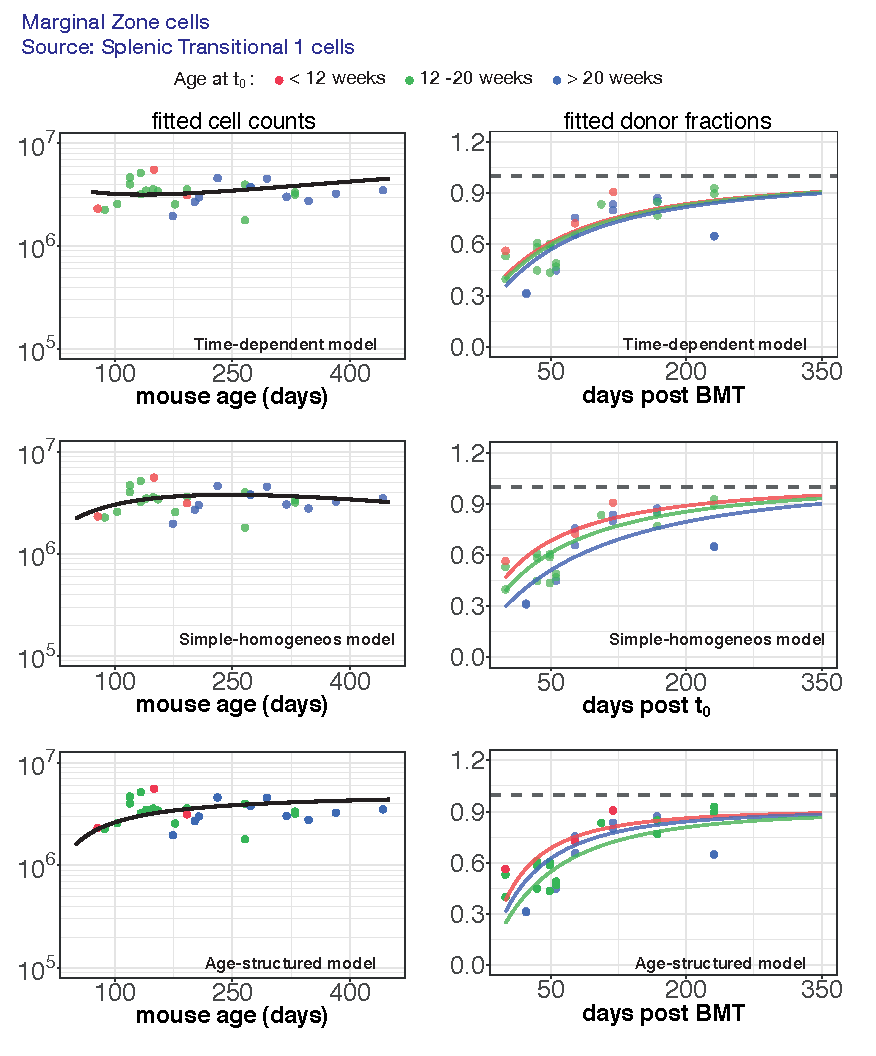
\includegraphics[scale = 1.1] {MZ_T1.pdf}}
	\caption{\small \textbf{Comparison of models  explaining dynamics of MZ B cells considering splenic T1 cells as precursors, in busulfan chimeras.} The time-dependent, simple-homogeneous and age-structured$^{\dagger}$ models fitted simultaneously to MZ cell counts and the normalised chimerism from busulfan chimeras made in recipients of different ages. Colours indicate different age-groups of recipient mice. The predictions shown were generated using the  mode of the age within each group.}
	\label{fig:MZ_T1}
\end{figure}

\begin{figure}[h!]
	\centerline{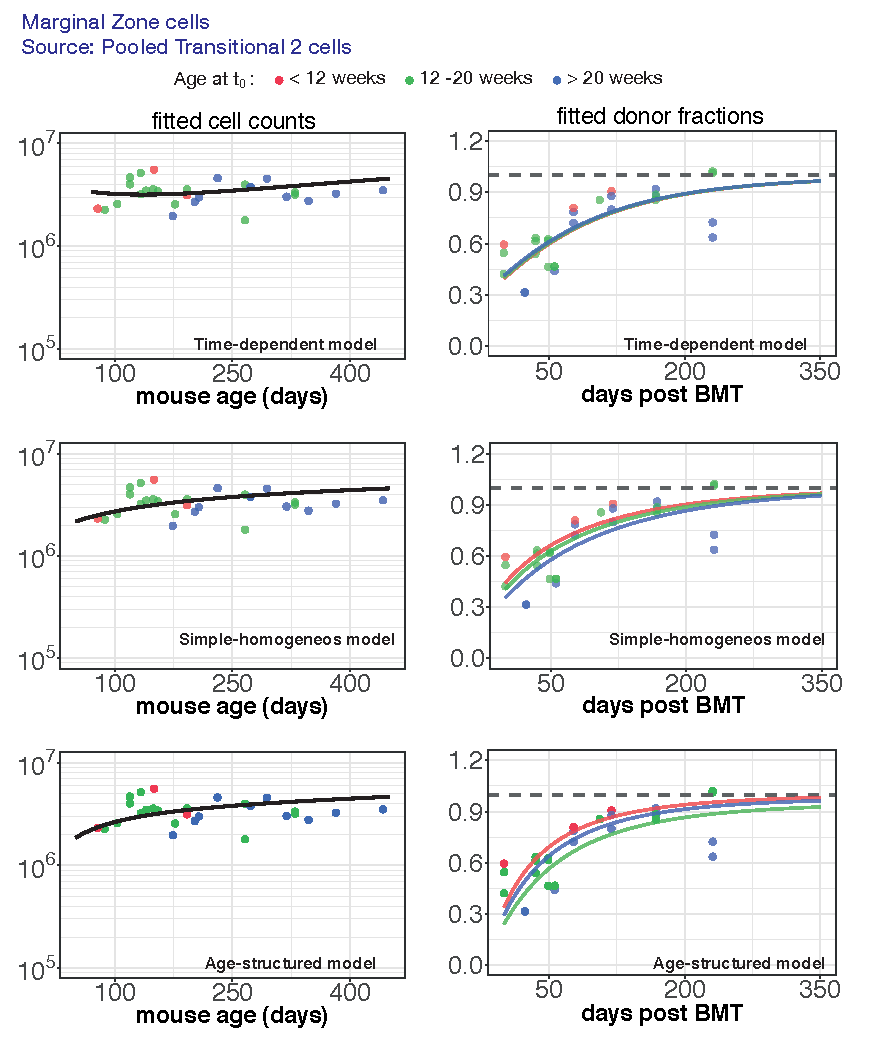
\includegraphics[scale = 1.1] {MZ_T2.pdf}}
	\caption{\small \textbf{Comparison of models  explaining dynamics of MZ B cells considering Pooled (spleen + LN) T2 cells as precursors, in busulfan chimeras.} The time-dependent, simple-homogeneous and age-structured$^{\dagger}$ models fitted simultaneously to MZ cell counts and the normalised chimerism from busulfan chimeras made in recipients of different ages. Colours indicate different age-groups of recipient mice. The predictions shown were generated using the  mode of the age within each group.}
	\label{fig:MZ_T2}
\end{figure}

%: Table MZ
\begin{table}[h!]
	\begin{center}
		\renewcommand{\arraystretch}{1.25}
		\begin{tabular}{ l c c c } 
			\toprule 
			\multicolumn{1}{l}{\textbf{MZ cells using}} & \multicolumn{3}{c}{\textbf{Model and $\Delta$AIC}} \\
			\cline{2-4}
			\textbf{Source}  &  {\small Time-dependent}  &  {\small Age-structured} & {\small Simple-homogeneous} \\ 
			\toprule
			Splenic Transitional 1 cells      & 0      &  6.94   & 4.86  \\ 
			Pooled Transitional 2 cells       & 7.90   &  9.99   & 6.11  \\
			\hline
			\toprule 
		\end{tabular}
	\end{center}
	\caption{\small Comparison of AIC values for different models fitted to cell counts and donor fractions$^{\dagger}$ in Marginal zone B cells, considering different precursor populations. }
	$^{\dagger}$ \footnotesize{Donor fractions in MZ pool were normlised to the donor fractions in the respective source population. }
	\label{tab:MZ-AICs}
\end{table} 





\clearpage

\begin{figure}[h!]
	\centerline{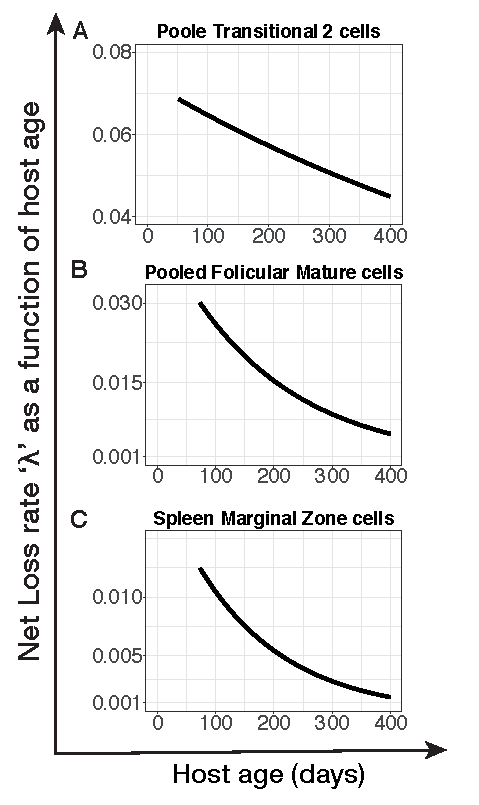
\includegraphics[scale = 1.1] {lambda_plots.pdf}}
	\caption{\small \textbf{Estimates of net loss rate $\lambda$ changing with time/host age from time-dependent model for (A) Pooled T2, (B) Pooled FM and for (C) Spleen MZ cells }}
	\label{fig:lambda}
\end{figure}


\section*{Inferring rates of division and loss using ki67 expression}
B cell subsets can be further divided in to recently divided (ki67Hi) and quiscent (ki67Lo) compartments. Dynamics of these compartments can  be tracked over time by studying changes in ki67 expression in the given subset and this information can be used to infer the rates of division and loss (death + maturation).

\begin{figure}[htbp]
	\centerline{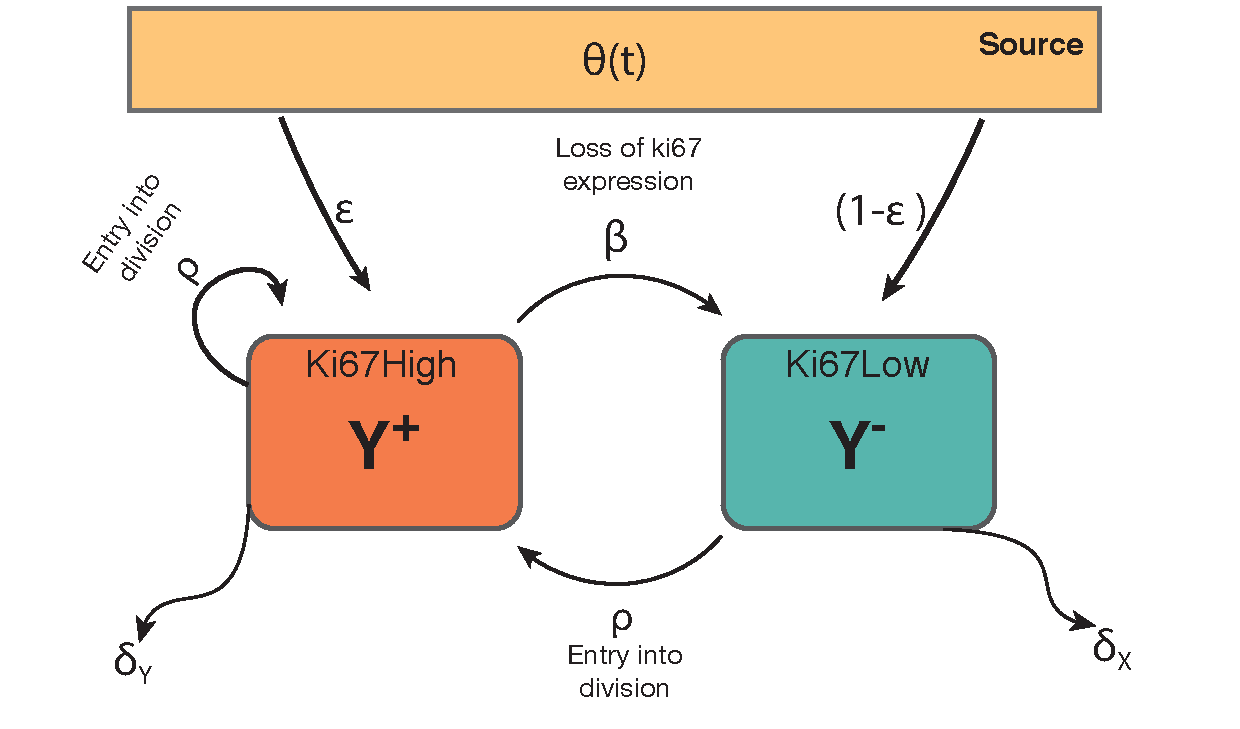
\includegraphics[scale = 0.5] {TwoComp_ki67.pdf}}
	\caption{Two compartment model for prolifeartion and loss of B cells using ki67 as a marker for dividing and recently divided cells \label{fig1}}
\end{figure}

This system is represented by the coupled ordinary differential equation described in eq.~\ref{general_ode}.

\begin{eqnarray}
\begin{aligned}
\frac{dY^+}{dt} &= \phi(t) \, \epsilon + \alpha \, (2\, Y^- + Y^+) - \beta Y^+ - \delta^+ Y^+ \\
\frac{dY^-}{dt} &= \phi(t) \, (1-\epsilon) - \alpha Y^-  + \beta Y^+ - \delta^- Y^+
\end{aligned}
\label{general_ode}
\end{eqnarray}

Where, $\epsilon$ denotes the proportions of ki67Hi cells within the source influx.

$\alpha$ - the rate of entry into division for both ki67Lo and ki67Hi cells.
Therefore, $\frac{1}{\alpha}$ is the time taken for individual cells to divide.

$\beta$ - the rate of loss of ki67 expression.
$\frac{1}{\beta}$ - the average time taken for ki67Hi cells to become ki67Lo.
We estimate $\frac{1}{\beta}$ from the experimental data which is 3.5 days. 

$\delta$ - the rate of loss (death + maturation) and it is possible that the ki67Hi and ki67Lo cells may have different susceptibility to die and/or mature.
We denote different rates $\delta_X$ and $\delta_Y$ for ki67Lo and ki67Hi cells respectively and assume a proportional relationship between these quantities, such that $\delta_Y = \sigma \, \delta_X$.

At $\sigma =1$, both ki67Hi and ki67Lo cells are lost at identical rates.
The resident times for individual cells within each compartment is given by, $\frac{1}{\delta}$.


We assumed that the influx from the source population changes very slowly relative to transition from ki67Hi to ki67Lo state, and therefore, both these compartments (X and Y) are in quasi-equilibrium. By equating eq.~\ref{general_ode} to either eq.~\ref{eq:SHM} or \ref{eq:TDM} or \ref{eq:ASM}, depending on the model. Therefore, considering the relationship `$\lambda = \delta - \rho$'; rates of division ($\rho$) and loss ($\delta$) can be inferred.


\bea
\begin{aligned}
\rho &= \frac{\kappa \, (1+ \kappa \, (\sigma -1)) + (\lambda \, \tau \, (\epsilon + \sigma) - \epsilon \, \sigma)) - (\lambda \, \tau \, \epsilon)}{\tau \, (1-\kappa) \, (2 + \kappa \, (\sigma -1))}\\
\\
\delta &= \frac{(1+\kappa \, (\sigma -1)) \, (\kappa + \lambda \, \tau \,(2-\epsilon - \kappa))}{\tau \, (1-\kappa) \, (2+\kappa \, (\sigma - 1))}
\end{aligned}
\label{rho_delta}
\eea

Where $\kappa$ is the measured fraction of ki67Hi cells. In subsets where $\kappa$ changes with time $\rho$ and $\delta$ will also change with time.
In time-dependent and age-structured models, changes in $\rho$ and $\delta$ over time are reflected in the variations in net loss rate $\lambda$ with time. 
However, the simple-homogeneous model considers that the net loss rate $\lambda$ is constant with time and forces changes in $\rho$ and $\delta$ to be linked to each other, such that for a relative decline in $\rho$ will impose an identical decline in $\delta$. Therefore, the simple-homogeneous model may not be compatible for subsets in which $\kappa$ changes with time, as it restricts the freesom in the model.


Based on this analysis it can be predicted that changes in ki67Hi proportions depend on, \\
(i) ki67Hi fraction in the influx i.e. $\epsilon$ and \\
(ii) Rates of division and loss of the population of interest. 


\begin{figure}[h!]
	\centerline{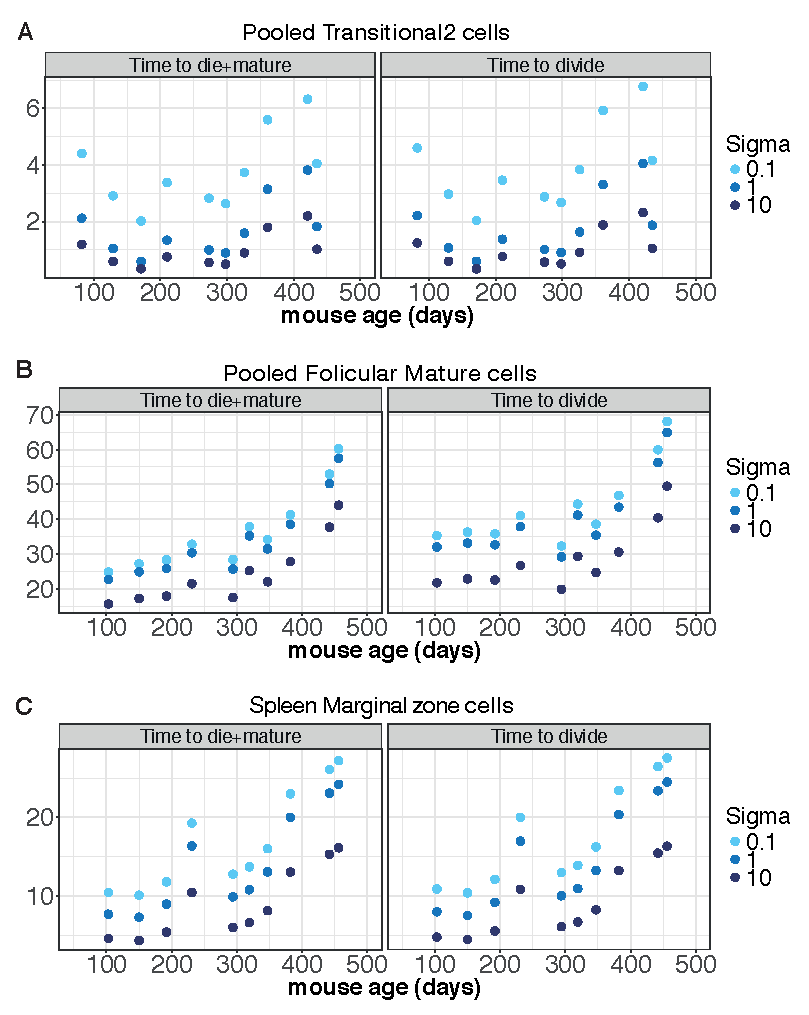
\includegraphics[scale = 1.1] {rate_estimates.pdf}}
	\caption{\small \textbf{Estimates of inter-division and residence time of B cell subsets.}  inter-division time (inverse of $\rho$) and residence time $\delta$ were estimated for B cell subsets using estimates of $\lambda$ and the ,measured values of $\kappa$ and $\epsilon$. Plots from the Best-fit models are only shown here: (For pooled FM - TDM with T1 as a source, for Spleen MZ - TDM with T1 as a source and for pooled T2 - TDM with T1 as a source). Colours indicate different values of sigma for which inverese of rates were estimated.}
	$^{\dagger}$ \footnotesize{For the time-dependent model, $\lambda(t)$ was estimated at the time points where $\kappa$ and $\epsilon$ are meausred which were then used to calculate $\frac{1}{\rho}$ and $\frac{1}{\delta}$.\\
	For the age-structure model, $\lambda(a)$ was integrated across all possible ages at the time points where $\kappa$ and $\epsilon$ are meausred. The values of lambda at specific timepoints were then used to calculate $\frac{1}{\rho}$ and $\frac{1}{\delta}$.}
	\label{fig:rates}
\end{figure}




\end{document}